\chapter{OSPF: Part 2}\label{ospf-part-2}

OSPF METRIC (Cost)

\begin{itemize}
\tightlist
\item
  OSPFs METRIC is called \textbf{COST}
\item
  It is automatically calculated based on the bandwidth (SPEED) of the
  INTERFACE
\item
  It is calculated by DIVIDING a REFERENCE BANDWIDTH value by the
  INTERFACE bandwidth
\item
  The DEFAULT REFERENCE BANDWIDTH is 100 mbps

  \begin{itemize}
  \tightlist
  \item
    REFERENCE: 100 mbps / INTERFACE: 10 mbps = COST (10)
  \item
    REFERENCE: 100 mbps / INTERFACE: 100 mbps = COST (1)
  \item
    REFERENCE: 100 mbps / INTERFACE: 1000 mbps = COST (1)
  \item
    REFERENCE: 100 mbps / INTERFACE: 10000 mbps = COST (1)
  \end{itemize}
\item
  ALL COST values less than 1 will be CONVERTED to 1
\item
  Therefore FastEthernet (100 mbps), Gigabit Ethernet (1000 mbps), 10
  Gig Ethernet, etc. are EQUAL and all have a COST of 1
\end{itemize}

FastEthernet COST

\begin{figure}
\centering
\pandocbounded{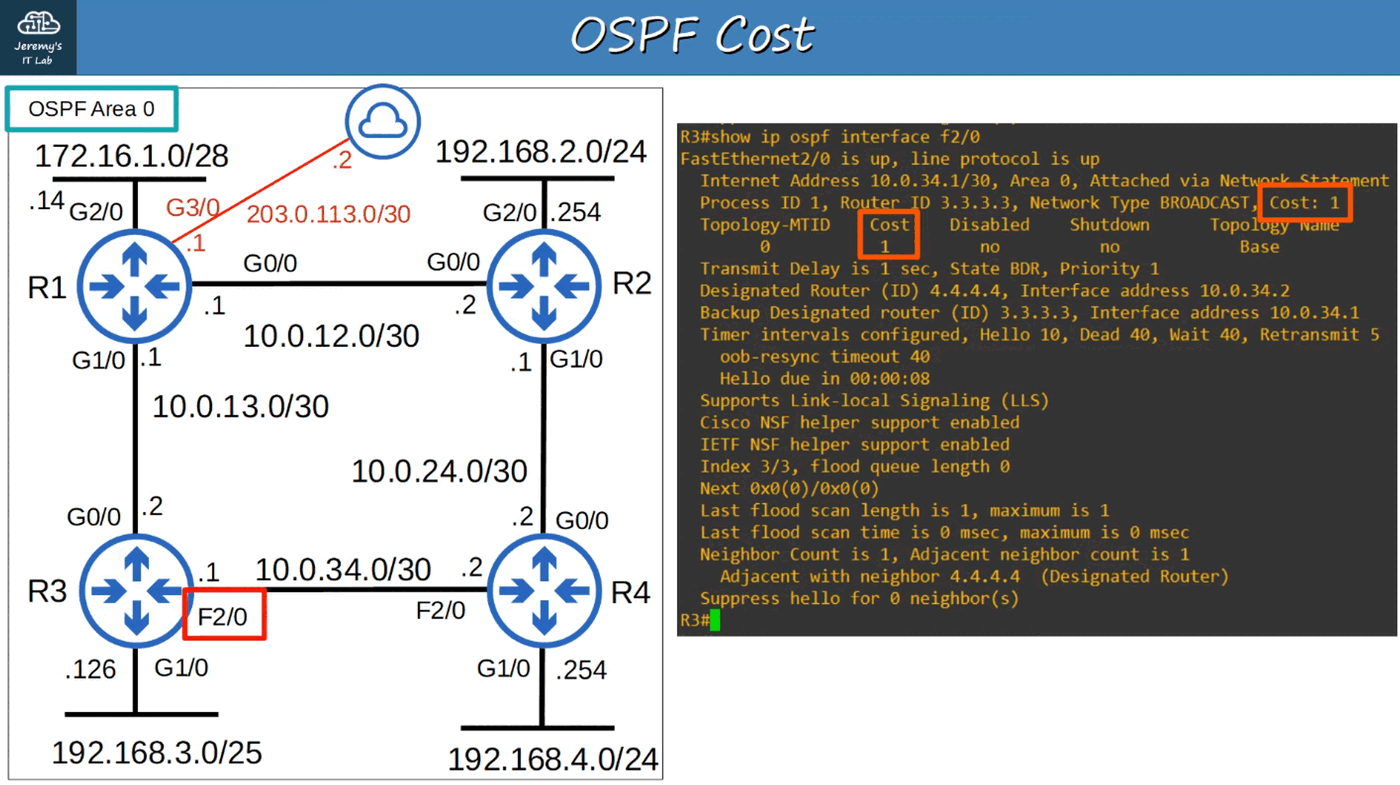
\includegraphics[keepaspectratio,alt={image}]{images/28-ospf-part2/img-001.png}}
\end{figure}

Gigabit Ethernet COST

\begin{figure}
\centering
\pandocbounded{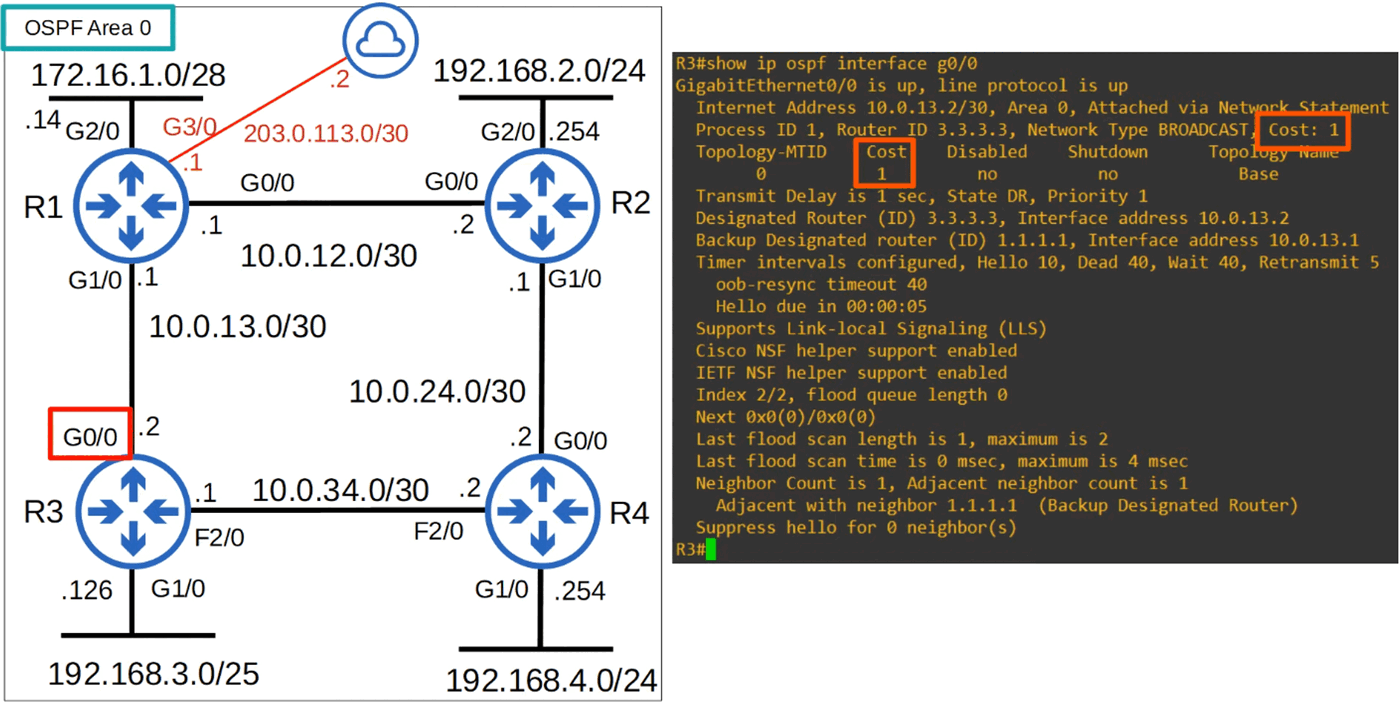
\includegraphics[keepaspectratio,alt={image}]{images/28-ospf-part2/img-002.png}}
\end{figure}

You can (and SHOULD) change the REFERENCE BANDWIDTH with this command:

R1(config-router)\# \textbf{auto-cost reference-bandwidth}
\emph{megabits-per-second}

The command is entered in ``megabits per second'' (DEFAULT is ``100'')

Example: using a value of ``100000''

\begin{itemize}
\tightlist
\item
  100000 / 100 = COST of 1000 for FastEthernet
\item
  100000 / 1000 = COST of 100 for Gig Ethernet
\end{itemize}

You should configure a reference bandwidth GREATER than the FASTEST
links in your NETWORK (to allow for future upgrades)

Changing the REFERENCE BANDWIDTH needs to be done on ALL OSPF ROUTERS in
the NETWORK

THE OSPF COST to a DESTINATION is the TOTAL COST of the `outgoing/exit
INTERFACES'

LOOPBACK INTERFACES have a COST of 1

\begin{figure}
\centering
\pandocbounded{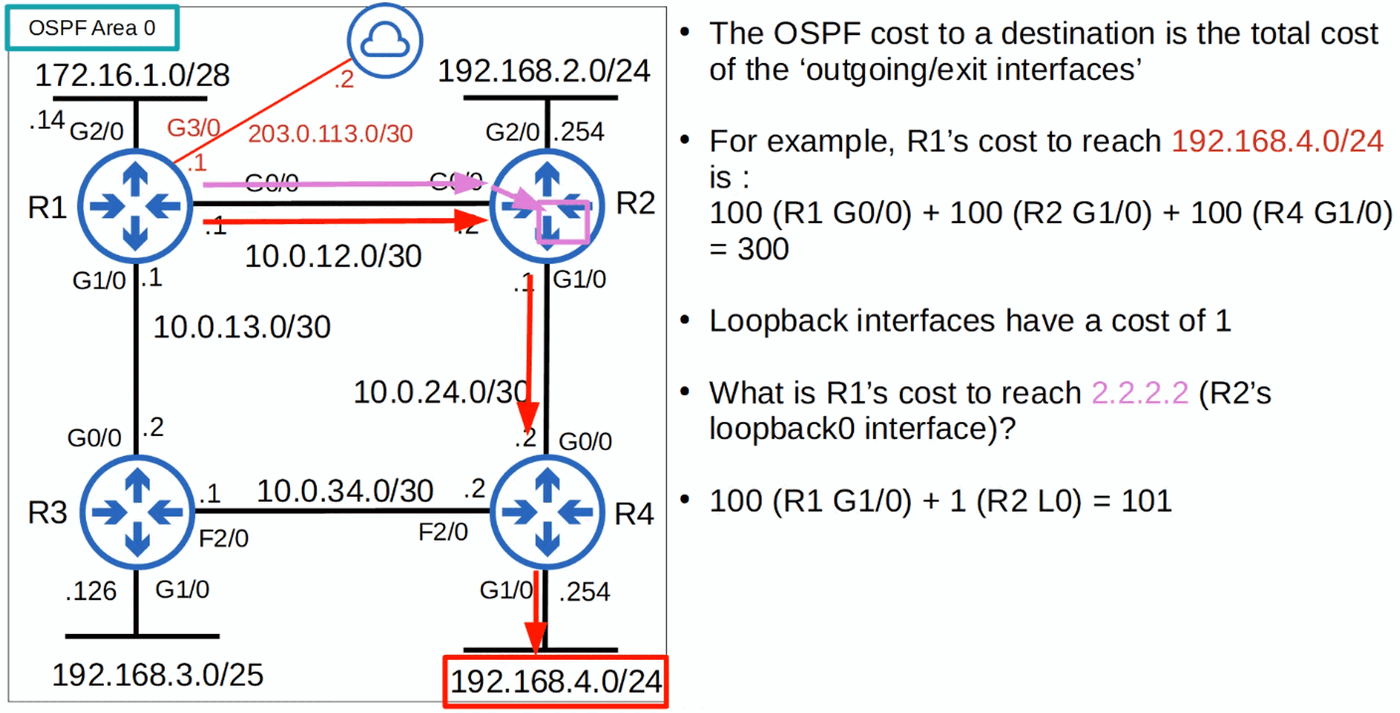
\includegraphics[keepaspectratio,alt={image}]{images/28-ospf-part2/img-003.png}}
\end{figure}

To CHANGE the OSPF COST of an INTERFACE, you use the command :

\begin{tipbox}

R1(config-if)\# ip ospf cost \textless cost\textgreater{}

\end{tipbox}

MANUAL COSTS take precedent over AUTOMATIC CALCULATED COST

One more option to change the OSPF COST of an INTERFACE is to change the
BANDWIDTH of the INTERFACE with the \textbf{``bandwidth''} command

The FORMULA to CALCULATE OSPF COST is :

\begin{tipbox}

\textbf{reference bandwidth / interface bandwidth}

\end{tipbox}

\begin{itemize}
\tightlist
\item
  Although the BANDWIDTH matches the INTERFACE SPEED (by DEFAULT),
  changing the INTERFACE BANDWIDTH \textbf{doesn't actually change the
  speed at which the INTERFACE operates}
\item
  The BANDWIDTH is just a VALUE that is used to calculate OSPF COST,
  EIGRP METRIC, etcetera\ldots{}
\item
  To CHANGE the SPEED at which the INTERFACE operates, use the
  \textbf{``speed''} command
\item
  Because the BANDWIDTH VALUE is used in other calculations, it is NOT
  recommended to change this VALUE to alter the INTERFACE's OSPF COST
\end{itemize}

It is RECOMMENDED that you CHANGE the REFERENCE BANDWIDTH

THEN use the \textbf{``ip ospf cost''} command to change the COST of the
individual INTERFACES, if you want.

\begin{figure}
\centering
\pandocbounded{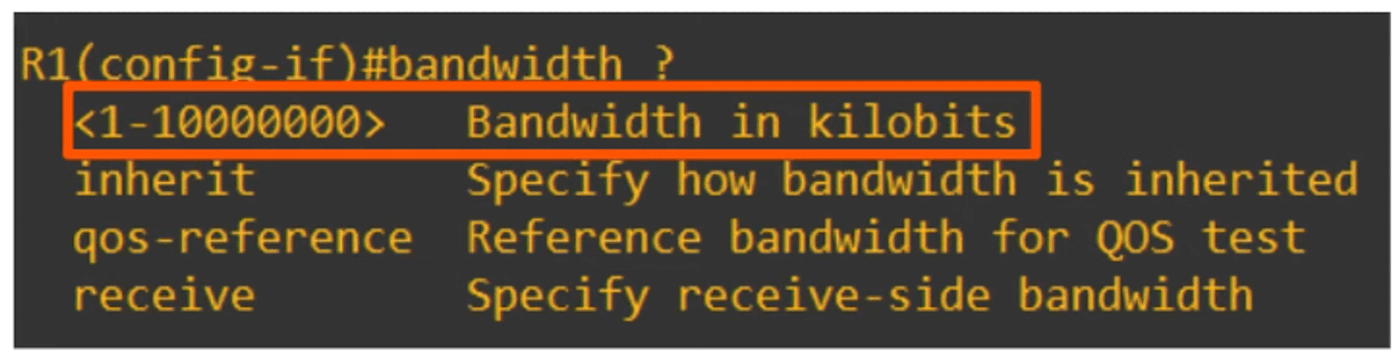
\includegraphics[keepaspectratio,alt={image}]{images/28-ospf-part2/img-004.png}}
\end{figure}

\section{Summary}\label{summary}

THREE WAYS to modify the OSPF COST:

\begin{enumerate}
\def\labelenumi{\arabic{enumi})}
\tightlist
\item
  Change the \textbf{\emph{reference bandwidth}}
\end{enumerate}

\begin{tipbox}

R1(config-router)\# \textbf{auto-cost reference-bandwidth}
\emph{megabits-per-second}

\end{tipbox}

\begin{enumerate}
\def\labelenumi{\arabic{enumi})}
\setcounter{enumi}{1}
\tightlist
\item
  Manual configuration:
\end{enumerate}

\begin{tipbox}

R1(config-router)\# ip ospf cost \textless cost\textgreater{}

\end{tipbox}

\begin{enumerate}
\def\labelenumi{\arabic{enumi})}
\setcounter{enumi}{2}
\tightlist
\item
  Change the \textbf{\emph{interface bandwidth}}
\end{enumerate}

\begin{tipbox}

R1(config-router)\# bandwidth
\textless kilobits-per-second\textgreater{}

\end{tipbox}

\begin{figure}
\centering
\pandocbounded{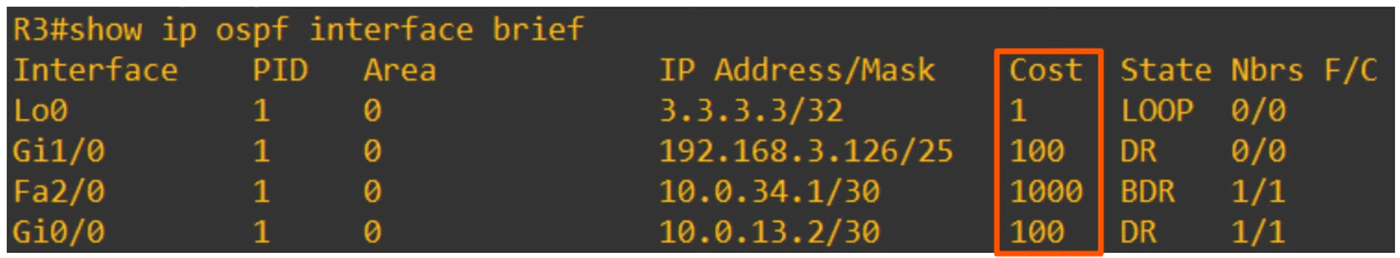
\includegraphics[keepaspectratio,alt={image}]{images/28-ospf-part2/img-005.png}}
\end{figure}

\section{Becoming OSPF Neighbors}\label{becoming-ospf-neighbors}

\begin{itemize}
\tightlist
\item
  Making sure that ROUTERS successfully become OSPF NEIGHBORS is the
  MAIN task in configuring and troubleshooting OSPF.
\item
  Once ROUTERS become NEIGHBORS, they AUTOMATICALLY do the work of
  sharing NETWORK information, calculating routes, etc.
\item
  When OSPF is activated on an INTERFACE, the ROUTER starts sending OSPF
  \textbf{``hello''} messages out of the INTERFACE at regular intervals
  (determined by the \textbf{``hello timer'').} These are used to
  introduce the ROUTER to potential OSPF NEIGHBORS
\item
  The DEFAULT ``\textbf{hello timer}'' is \textbf{10 SECONDS} on an
  Ethernet connection
\item
  \textbf{Hello} messages are MULTICAST to \textbf{224.0.0.5} (multicast
  address for ALL OSPF ROUTERS)
\item
  OSPF messages are ENCAPSULATED in an IP HEADER, with a \textbf{value
  of ``89''} in the PROTOCOL field.
\end{itemize}

\section{Down State}\label{down-state}

\begin{itemize}
\tightlist
\item
  OSPF is activated on R1s G0/0 INTERFACE
\item
  It sends an OSPF ``hello'' message to 224.0.0.5
\item
  It doesn't know about any OSPF neighbors yet, so the current neighbor
  state is DOWN
\end{itemize}

\begin{figure}
\centering
\pandocbounded{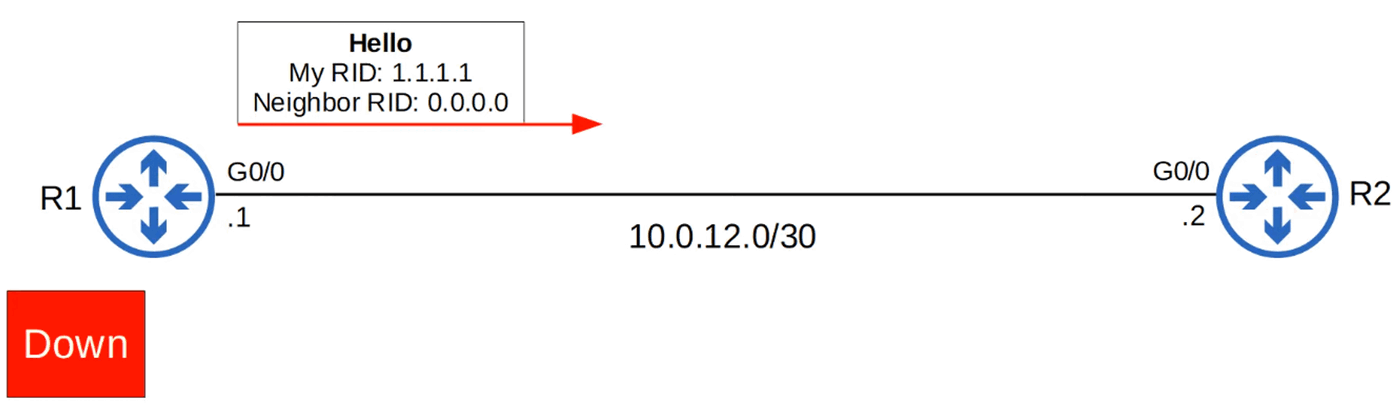
\includegraphics[keepaspectratio,alt={image}]{images/28-ospf-part2/img-006.png}}
\end{figure}

\section{Init State}\label{init-state}

\begin{itemize}
\tightlist
\item
  When R2 receives the ``hello'' packet, it will add an entry for R1 to
  its OSPF neighbor table
\item
  In R2's neighbor table, the relationship with R1 is now in the INIT
  state
\item
  INIT state = ``hello'' packet received, but own ROUTER ID is not in
  the ``hello'' packet
\end{itemize}

\begin{figure}
\centering
\pandocbounded{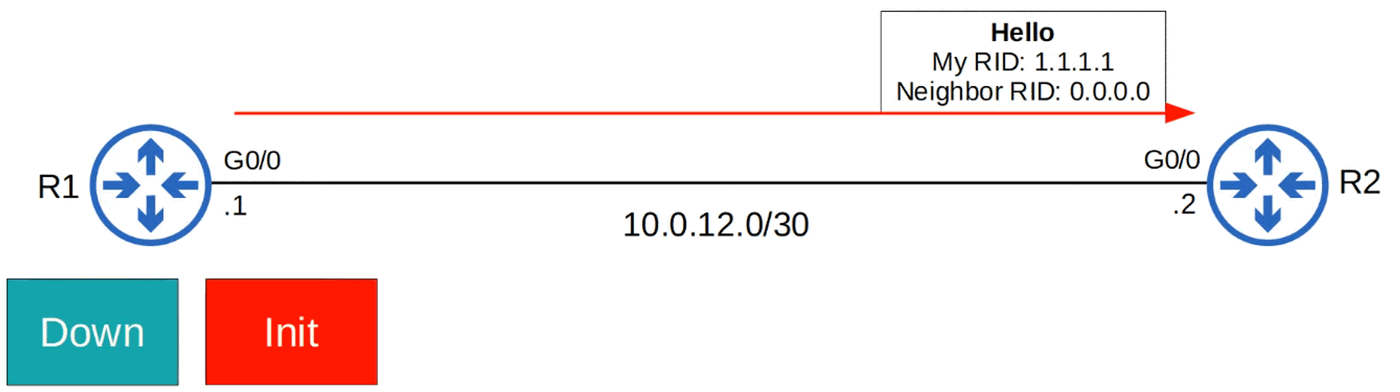
\includegraphics[keepaspectratio,alt={image}]{images/28-ospf-part2/img-007.png}}
\end{figure}

2-WAY STATE

\begin{itemize}
\tightlist
\item
  R2 will send a ``hello'' packet containing the RID of BOTH ROUTERS
\item
  R1 will insert R2 into its OSPF neighbor table in the 2-WAY state
\item
  R1 will send another ``hello'' message, this time containing R2's RID
\item
  Both ROUTERS are now in the 2-WAY state
\end{itemize}

\begin{figure}
\centering
\pandocbounded{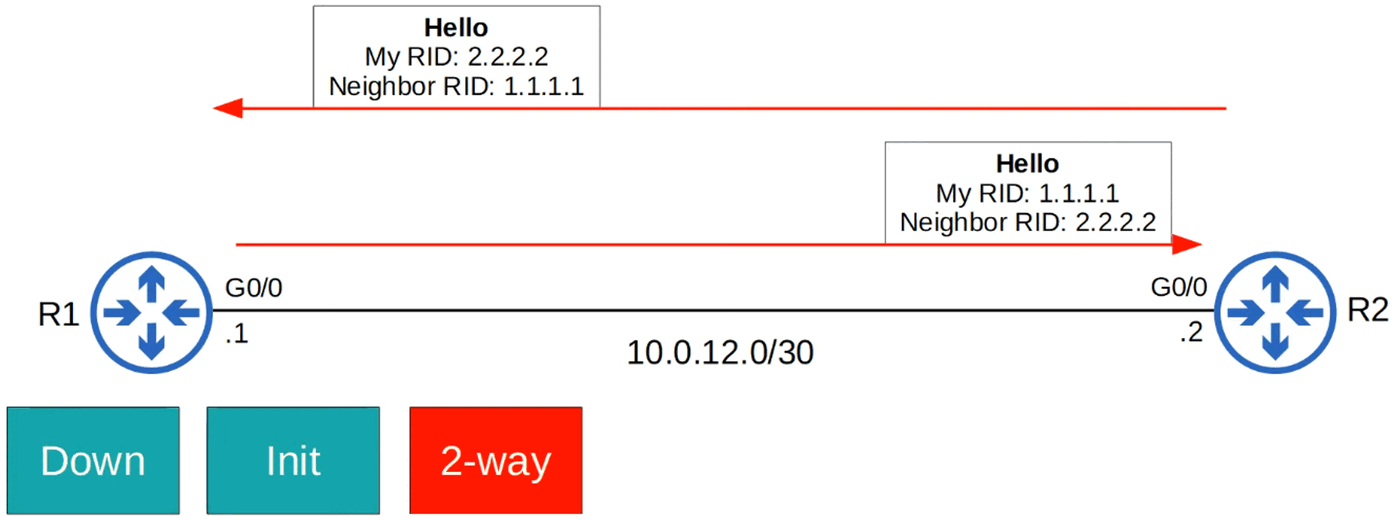
\includegraphics[keepaspectratio,alt={image}]{images/28-ospf-part2/img-008.png}}
\end{figure}

\begin{itemize}
\tightlist
\item
  The 2-WAY state means the ROUTER has received a ``hello'' packet with
  its own RID in it
\item
  If both ROUTERS reach the 2-WAY state, it means that ALL of the
  conditions have been met for them to become OSPF neighbors.
\item
  They are now READY to SHARE LSAs to build a common LSDB.
\item
  In SOME NETWORK types, a DR (Designated ROUTER) and BDR (Backup
  Designated Router) will be elected at this point (OSPF Network Types
  and DR/DBR elections will be discussed in Day 28)
\end{itemize}

\section{ExStart State}\label{exstart-state}

\begin{itemize}
\tightlist
\item
  The TWO ROUTERS will now prepare to exchange information about their
  LSDB
\item
  Before that, they have to choose which one will START the exchange
\item
  They do THIS in the EXSTART state

  \begin{itemize}
  \tightlist
  \item
    The ROUTER with the higher RID will become the MASTER and initiate
    the exchange.
  \item
    The ROUTER with the lower RID will become the SLAVE
  \end{itemize}
\item
  To decide the MASTER and SLAVE, they exchange DBD (Database
  Description) packets
\end{itemize}

\begin{figure}
\centering
\pandocbounded{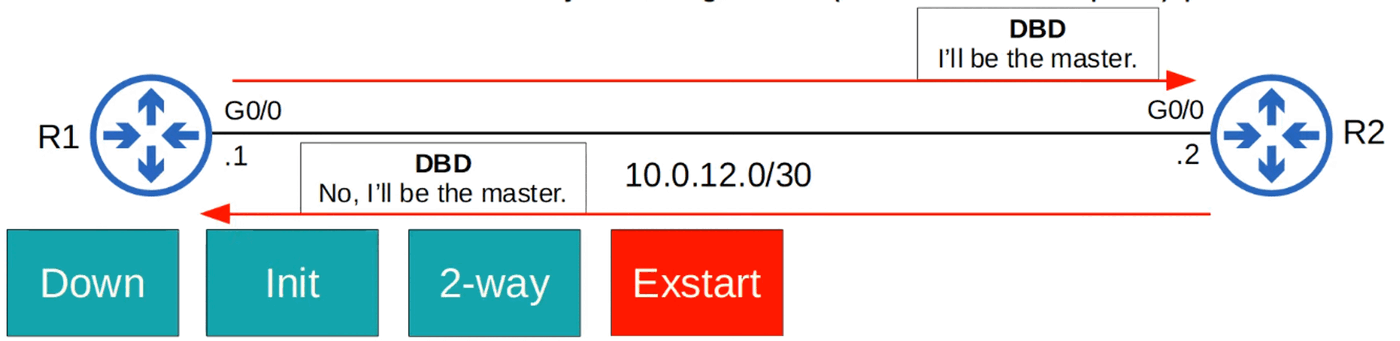
\includegraphics[keepaspectratio,alt={image}]{images/28-ospf-part2/img-009.png}}
\end{figure}

\section{Exchange State}\label{exchange-state}

\begin{itemize}
\tightlist
\item
  In the EXCHANGE state, the ROUTERS exchange DBDs which contain a LIST
  of the LSAs in their LSDB
\item
  These DBDs do NOT include detailed information about the LSAs, just
  BASIC INFORMATION
\item
  The ROUTERS compare the information in the DBD they received to the
  information in their OWN LSDB to determine which LSAs they must
  receive from their neighbor
\end{itemize}

\begin{figure}
\centering
\pandocbounded{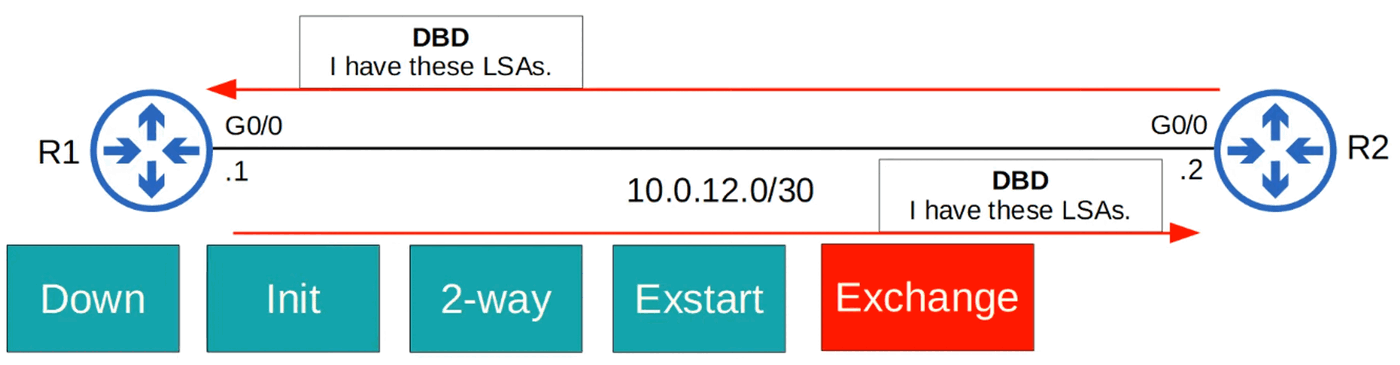
\includegraphics[keepaspectratio,alt={image}]{images/28-ospf-part2/img-010.png}}
\end{figure}

\section{Loading State}\label{loading-state}

\begin{itemize}
\tightlist
\item
  In the LOADING state, ROUTERS send \textbf{Link State Requests (LSR)}
  messages to request that their neighbors SEND them any LSAs they don't
  have
\item
  LSAs are sent in \textbf{Link State Update (LSU)} messages
\item
  The ROUTERS send \textbf{LSAck} messages to acknowledge that they
  received the LSAs
\end{itemize}

\begin{figure}
\centering
\pandocbounded{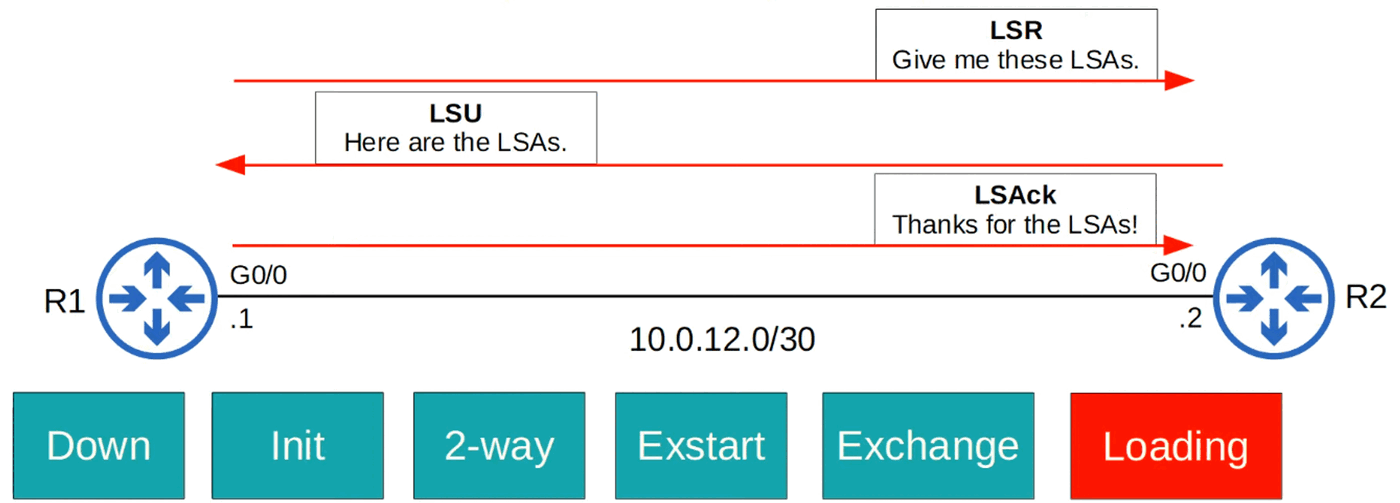
\includegraphics[keepaspectratio,alt={image}]{images/28-ospf-part2/img-011.png}}
\end{figure}

\section{Full State}\label{full-state}

\begin{itemize}
\tightlist
\item
  In the FULL state, the ROUTERS have a FULL OSPF adjacency and
  identical LSDBs
\item
  They continue to SEND and LISTEN for ``hello'' packets (every 10
  seconds by default) to maintain the neighbor adjacency
\item
  Every time a ``hello'' packet is received, the ``DEAD'' timer (40
  seconds by default) is reset
\item
  If the DEAD timer counts down to 0 and no ``hello'' message is
  received, the neighbor is REMOVED
\item
  The ROUTERS will continue to share LSAs as the network changes to make
  sure each ROUTER has a COMPLETE and ACCURATE map of the NETWORK (LSDB)
\end{itemize}

\begin{figure}
\centering
\pandocbounded{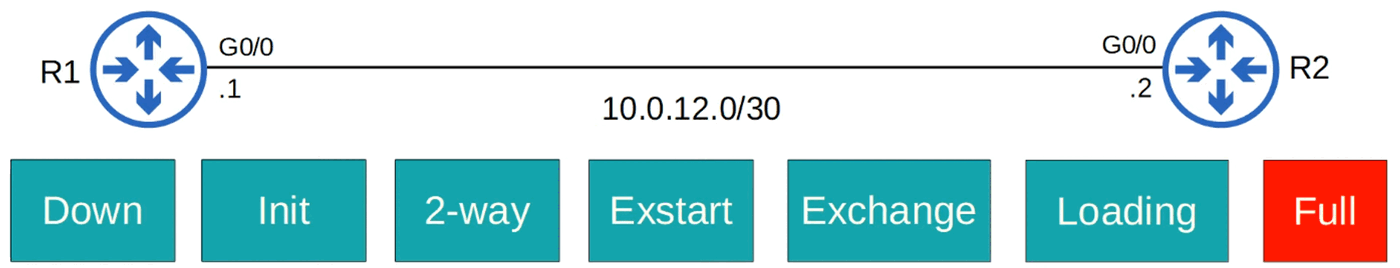
\includegraphics[keepaspectratio,alt={image}]{images/28-ospf-part2/img-012.png}}
\end{figure}

\section{OSPF Neighbors Summary}\label{ospf-neighbors-summary}

\begin{figure}
\centering
\pandocbounded{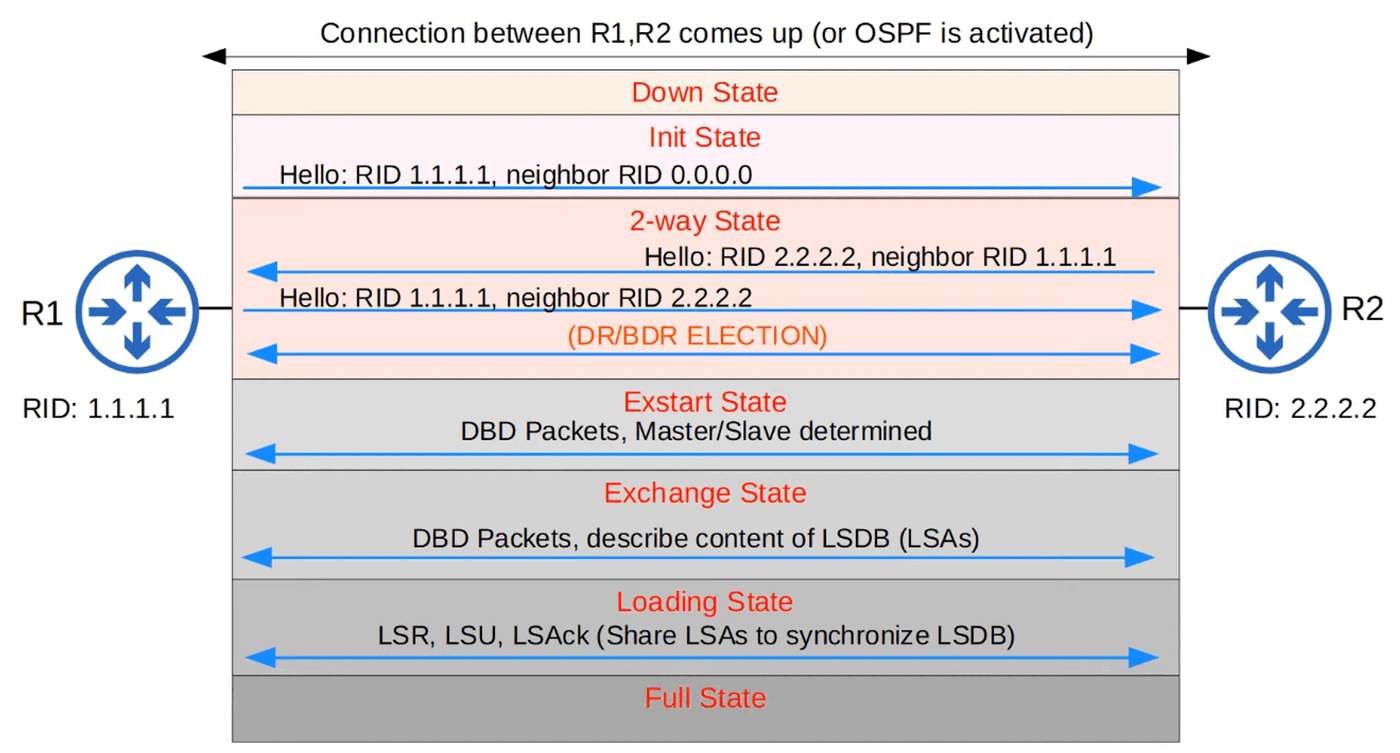
\includegraphics[keepaspectratio,alt={image}]{images/28-ospf-part2/img-013.png}}
\end{figure}

1 ) BECOME NEIGHBORS

\begin{itemize}
\tightlist
\item
  DOWN STATE
\item
  INIT STATE
\item
  2-WAY STATE
\item
  (DR/BDR ELECTION)
\end{itemize}

\begin{enumerate}
\def\labelenumi{\arabic{enumi})}
\setcounter{enumi}{1}
\tightlist
\item
  EXCHANGE LSAs
\end{enumerate}

\begin{itemize}
\tightlist
\item
  EXSTART STATE
\item
  EXCHANGE STATE
\item
  LOADING STATE
\end{itemize}

\section{Summary of OSPF Message
Types}\label{summary-of-ospf-message-types}

\begin{figure}
\centering
\pandocbounded{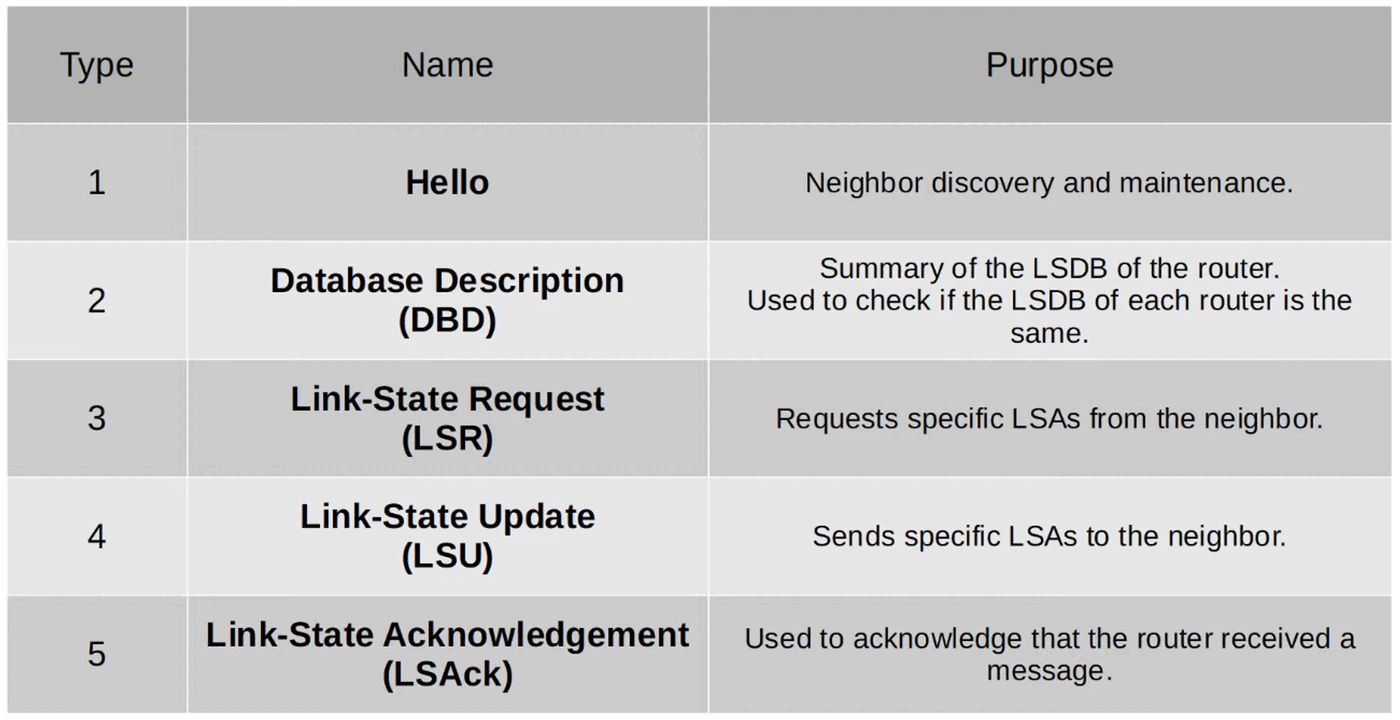
\includegraphics[keepaspectratio,alt={image}]{images/28-ospf-part2/img-014.png}}
\end{figure}

\section{More OSPF Configurations}\label{more-ospf-configurations}

Activate OSPF DIRECTLY on an INTERFACE with this command:

\begin{tipbox}

R1(config-if)\# ip ospf \emph{process-id} area \emph{area}

\end{tipbox}

\begin{figure}
\centering
\pandocbounded{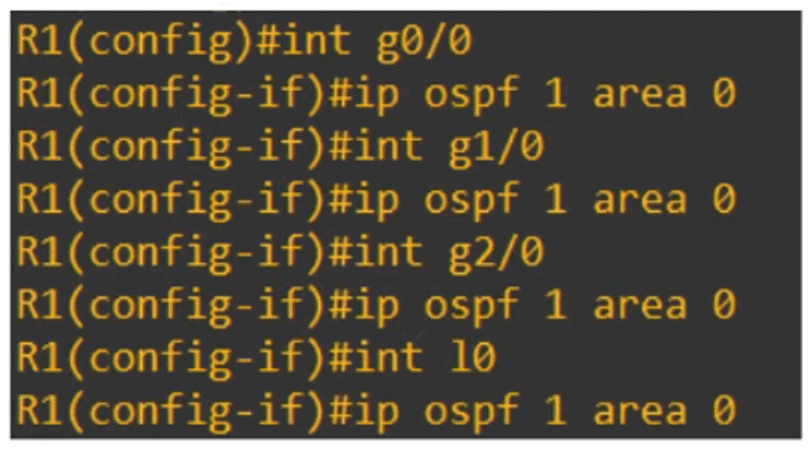
\includegraphics[keepaspectratio,alt={image}]{images/28-ospf-part2/img-015.png}}
\end{figure}

Configure ALL INTERFACES as OSPF Passive Interfaces

\begin{tipbox}

R1(config-router) \#passive-interface default

\end{tipbox}

\begin{figure}
\centering
\pandocbounded{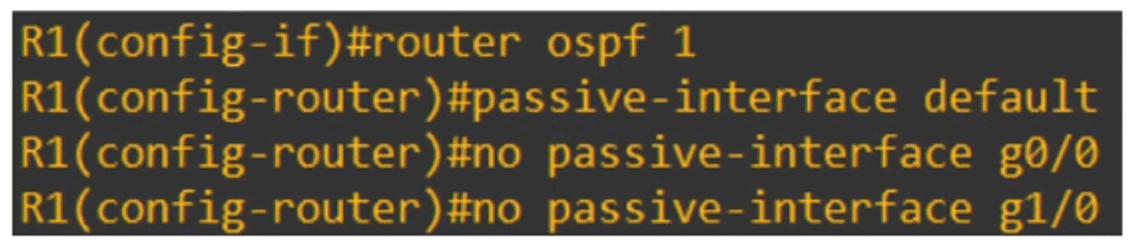
\includegraphics[keepaspectratio,alt={image}]{images/28-ospf-part2/img-016.png}}
\end{figure}

Can then REMOVE specific INTERFACES from being passive using:

\begin{tipbox}

R1(config-router) \#no passive-interface \emph{interface-id}

\end{tipbox}

Activating OSPF DIRECTLY on INTERFACES will show a different output in
``show ip protocols''

\begin{figure}
\centering
\pandocbounded{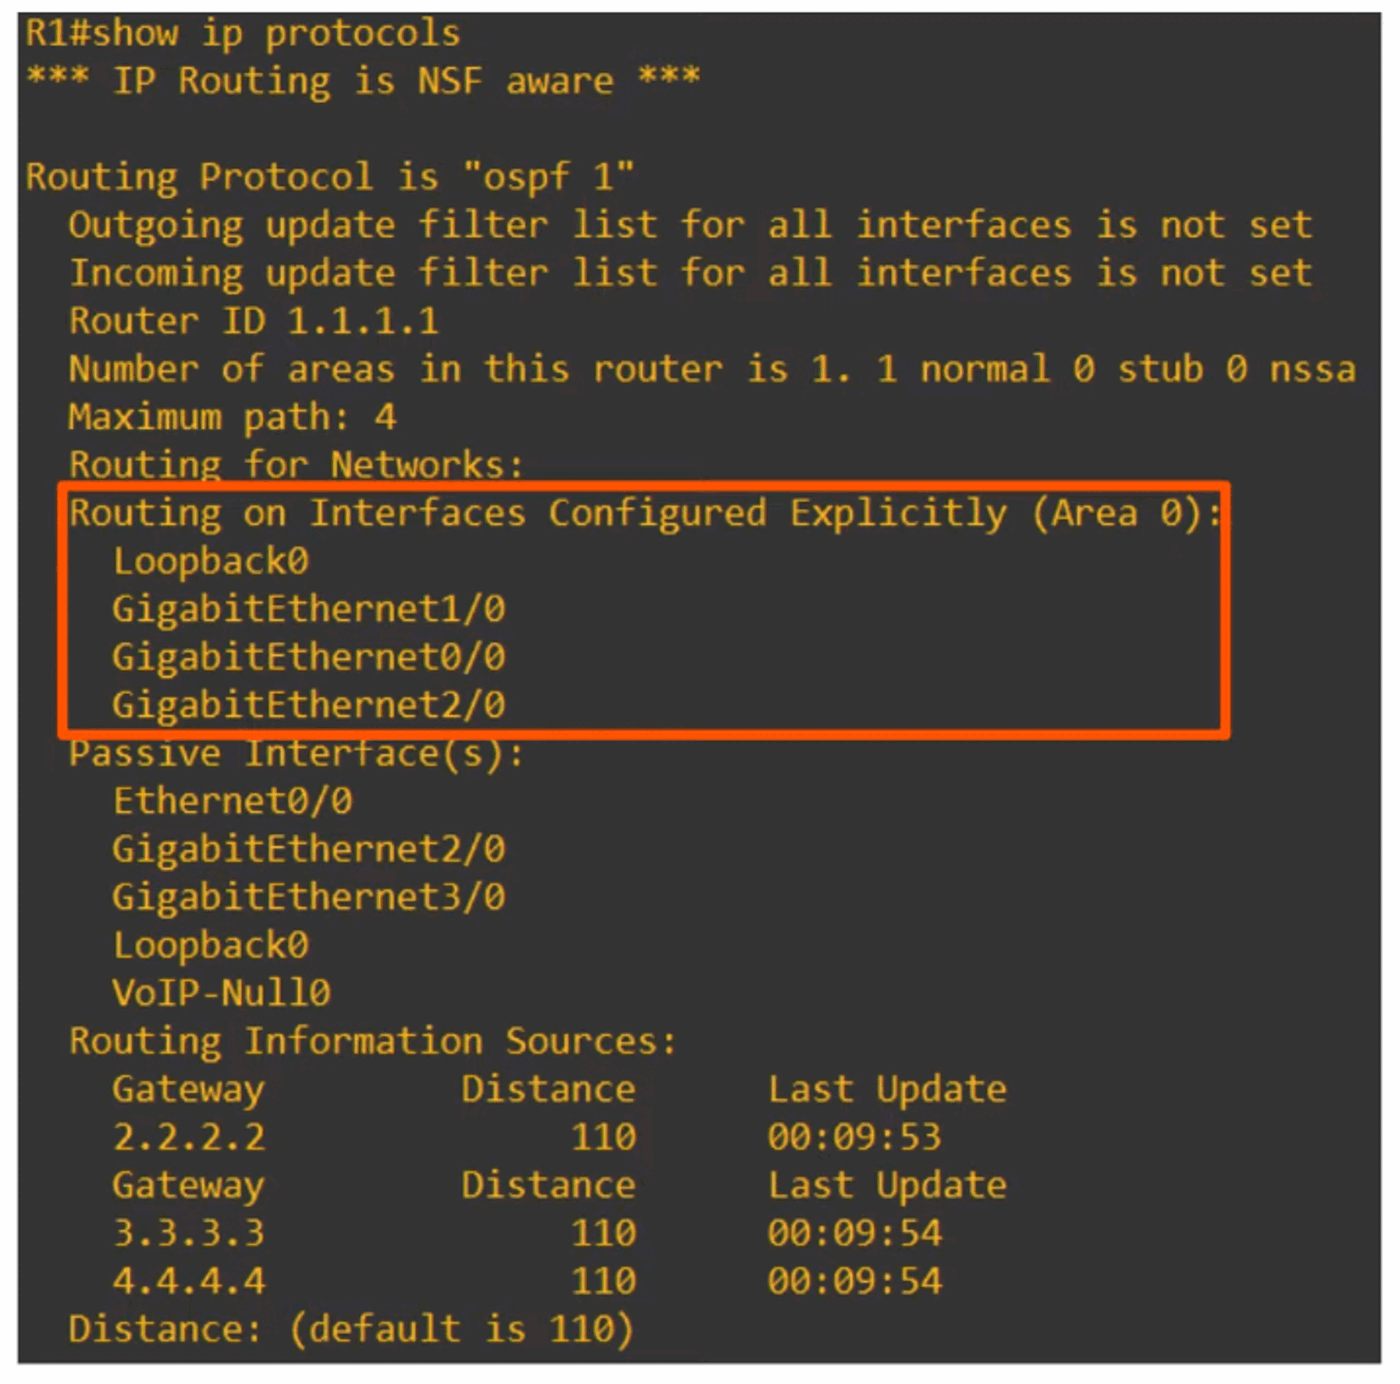
\includegraphics[keepaspectratio,alt={image}]{images/28-ospf-part2/img-017.png}}
\end{figure}

They will appear under ``Routing on Interfaces Configured Explicitly
(Area \#) :'' (as above)

Showing the OSPF LSDB of a Device

\begin{figure}
\centering
\pandocbounded{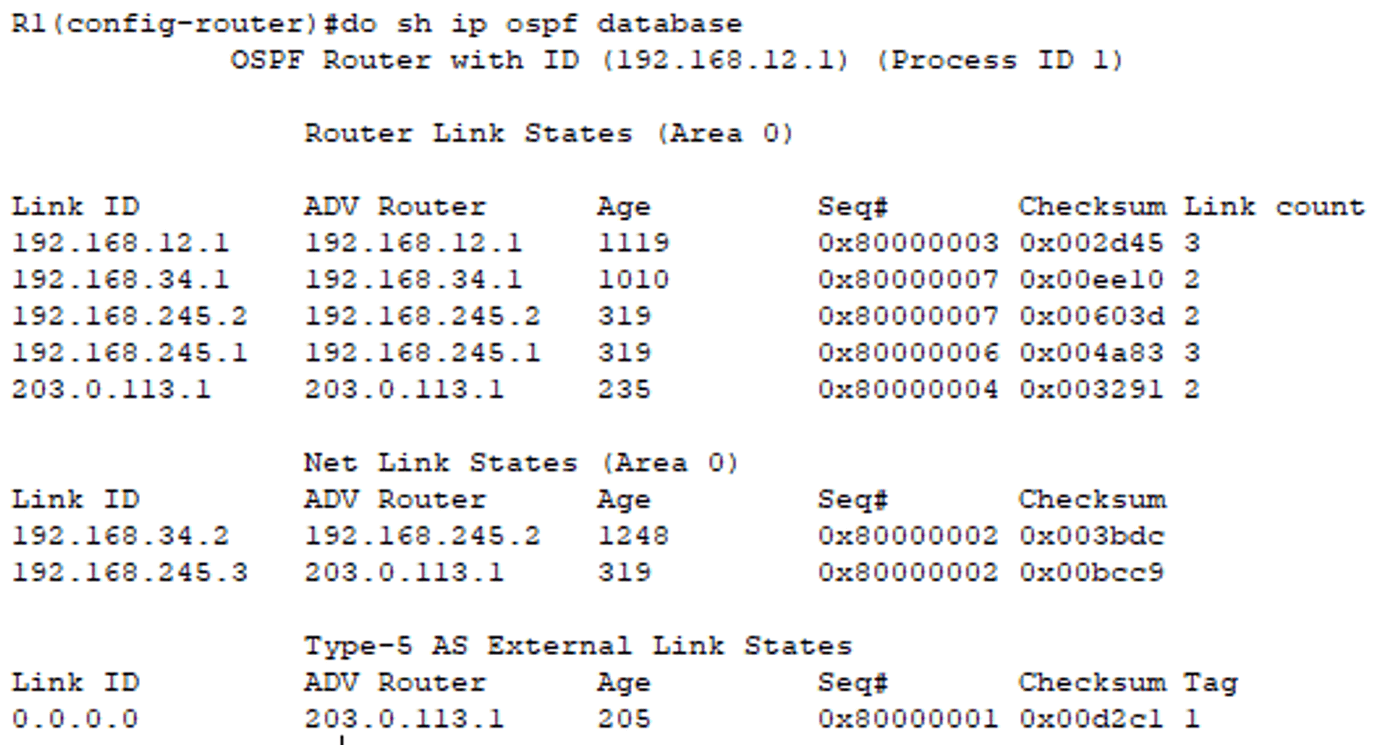
\includegraphics[keepaspectratio,alt={image}]{images/28-ospf-part2/img-018.png}}
\end{figure}
